\chapter{Research Method}
\label{methods}
Research methods, according to Jane et al. \cite{qualitateiveresearch2012}, are approaches, procedures and guidelines that are applied to conduct research, e.g., observation, interview, prototyping, experiment, etc. In this research, two main factors have driven the selection of research methods: i) the fact that the research is applied in industry (or involves industry-academia collaboration), which means the research results as well as the process should consider the interest and the nature of the industry, and ii) seamless integration of formal methods into existing engineering methods and practices with minimal cost, which requires careful consideration of existing engineering methods, guidelines, tools and capabilities. To summarize the main problems raised by the industry-academia collaboration: i) the research goals should target existing problems in the industry; ii) existing methods and tools should be leveraged; iii) proposed ideas, methods and tools should be agreed by both academia and industry teams before their design, implementation, validation, and integration to ensure usefulness; iv) furthermore, it is imperative that the proposed tools and methods are engineering-friendly, which means the research team is required to communicate with the actual users to capture the feel of the proposed methods and tools. 
\begin{figure}[h]
	\centering
	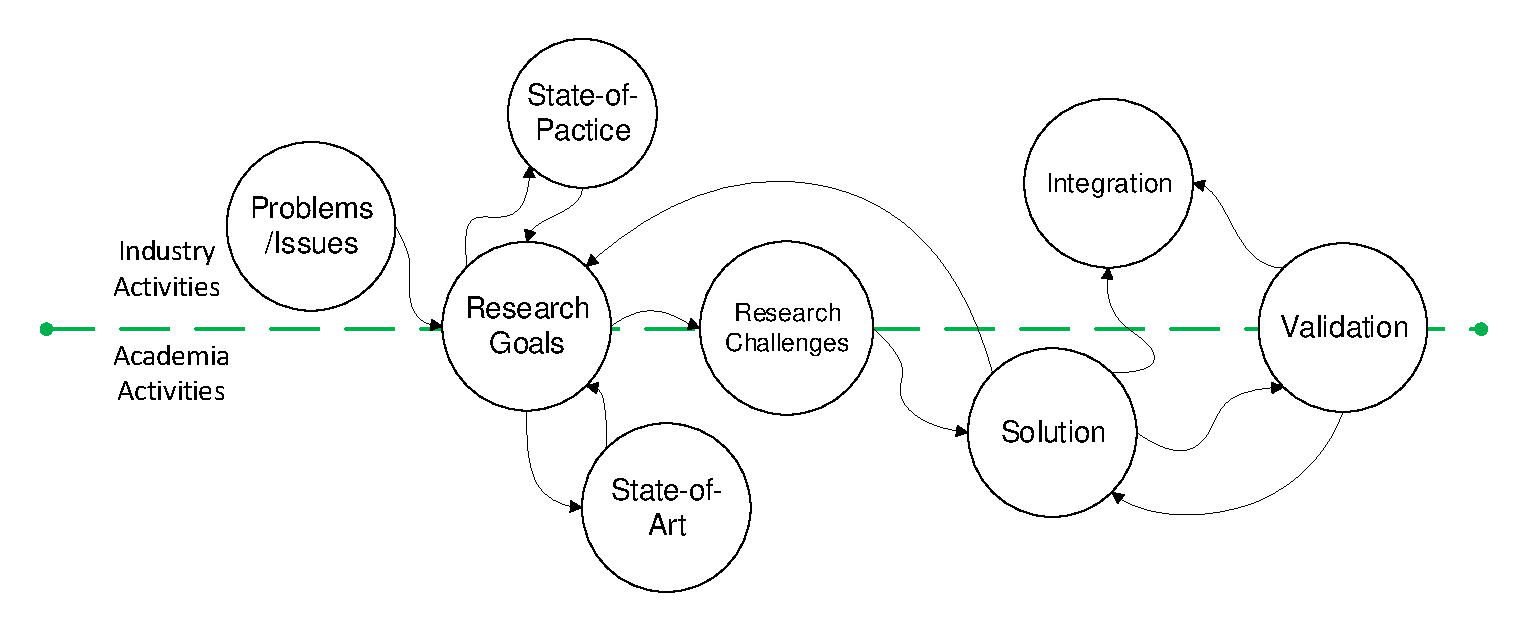
\includegraphics[trim=10 0 10 0, clip,width=1\linewidth]{images/research_process.pdf}
	\caption{Research Process.}
	\label{fig_research_process}
\end{figure}

Figure \ref{fig_research_process} illustrates the research process employed in the thesis, which is an adaptation of the technology-transfer process proposed by Tony et al. \cite{Gorschek2006APractice}. Our main research activities has involved identification of research goals and research challenges, which are followed by solution proposals and their implementations. Subsequently, the solutions are validated on industrial use cases, and are also integrated seamlessly into industrial tool chains. In order to conduct these activities, several quantitative and qualitative research methods are blended in order to gather, analyze and interpret, respectively, quantitative and qualitative data via what is known as \textit{hybrid (or mixed) research} \cite{Creswell2014ResearchApproaches}. The benefit of applying mixed research methods is mainly in the triangulation of research outcomes through various research methodical approaches. In fact, this can be better explained by the requirements specification research problem, which has accommodated empirical research via interview, observation to collect quantitative data that has allowed us to understand the current practices and needs of VGTT. Subsequently, we have proposed the ReSA framework, which have been validated through quantitative methods including statistical analysis and questionnaire on its effectiveness and usability\footnote{Work in progress - validation of the ReSA toolchain by practitioners, at VGTT.}.

During implementations of the proposed solutions, we have applied a prototyping method \cite{Carr2004PrototypingApproaches}, which has enabled incremental development of the solutions, before introducing grand progress in subsequent development phases, via concept modeling, implementation, demonstration and revision. This has been the case during the implementation of the ReSA framework \cite{resatool,Mahmud2017SpecificationLogic} as well as the SIMPPAAL framework \cite{Filipovikj2016SimulinkSystems}. The prototyping has involved concept development, and experimentation with toy examples and use cases to internally validate the implementation solutions, before validation by practitioners. Of course, the implementation of the research process has not been straightforward; on the contrary, similar to other research activities, it has accommodated several iterative, cyclic activities to clarify research goals and update solutions based on knowledge gained via literature study and feedback from industry.  Besides, the industrial flavor of the research has required persistent synchronization meetings through discussions and workshops in order to update to the state-of-the-art and state-of-the-practice methods and tools.
% \begin{figure} 
% \centering

%   	\includegraphics[trim=20 0 20 0, clip, width=0.7\linewidth]{research_method_activity.pdf}
%     \caption{Activity Diagram of the Research Process.}
%     \label{fig_discrete_block_ta}
%   \label{fig_ta}
% \end{figure}
